\documentclass[9pt]{beamer}


\usepackage{amsmath,amsfonts,amssymb,amsthm, gensymb}
\DeclareMathAlphabet{\mathbbold}{U}{bbold}{m}{n}    

\usepackage[utf8]{inputenc}
 

%Information to be included in the title page:
\title{A Parallel in Time Method for Optimal Control}
\subtitle{Parareal-Based preconditioner for BFGS algorithm}
\author{Andreas Thune}
\date{2017}
 
\usetheme{Berlin}
\usecolortheme{beaver}
\begin{document}
 
\frame{\titlepage}
\tableofcontents
\section{Problem}

\begin{frame}
\frametitle{Optimization with ODE constraints}
\begin{itemize}
\item{The aim of the thesis is to propose a parallel in time method for solving optimal control problems.}
\item{Our proposed algorithm uses a Parareal-based preconditioner originally introduced in [Maday et al] }
\end{itemize}
\begin{block}{Optimal Control Problem}
\begin{align*}
\min_{y,v} &J(y(t),v), \\
\textrm{subject to} \ &E(y(t),v)=0\quad t\in[0,T]
\end{align*}
\end{block}
\end{frame}
\begin{frame}
\frametitle{The Parareal algorithm}
\begin{columns}
\column{0.58\linewidth}
\begin{itemize}
\item{The Parareal algorithm was introduced in [Lion et al] as a way of parallelizing time-dependent PDEs $f(y(t),t)=0$ in temporal direction.}
\item{The Parareal algorithm combines a coarse and a fine numerical scheme for a discretization in time. The fine scheme is run in parallel, while the coarse scheme is run serially.}
\item{If we let $\bold{F}_{\Delta T}$ and $\bold{G}_{\Delta T}$ be the fine and coarse propagators that evolve the equation from $\lambda$ at time $t$ to $y(t+\Delta T)$, the Parareal algorithm can be stated as the following iteration:
\begin{align*}
\lambda_{i+1}^{k+1} = \bold{G}_{\Delta T}(\lambda_{i}^{k+1})+\bold{F}_{\Delta T}(\lambda_{i}^{k})-\bold{G}_{\Delta T}(\lambda_{i}^{k})
\end{align*}}

\end{itemize}
\column{0.48\linewidth}
\begin{figure}[!h]
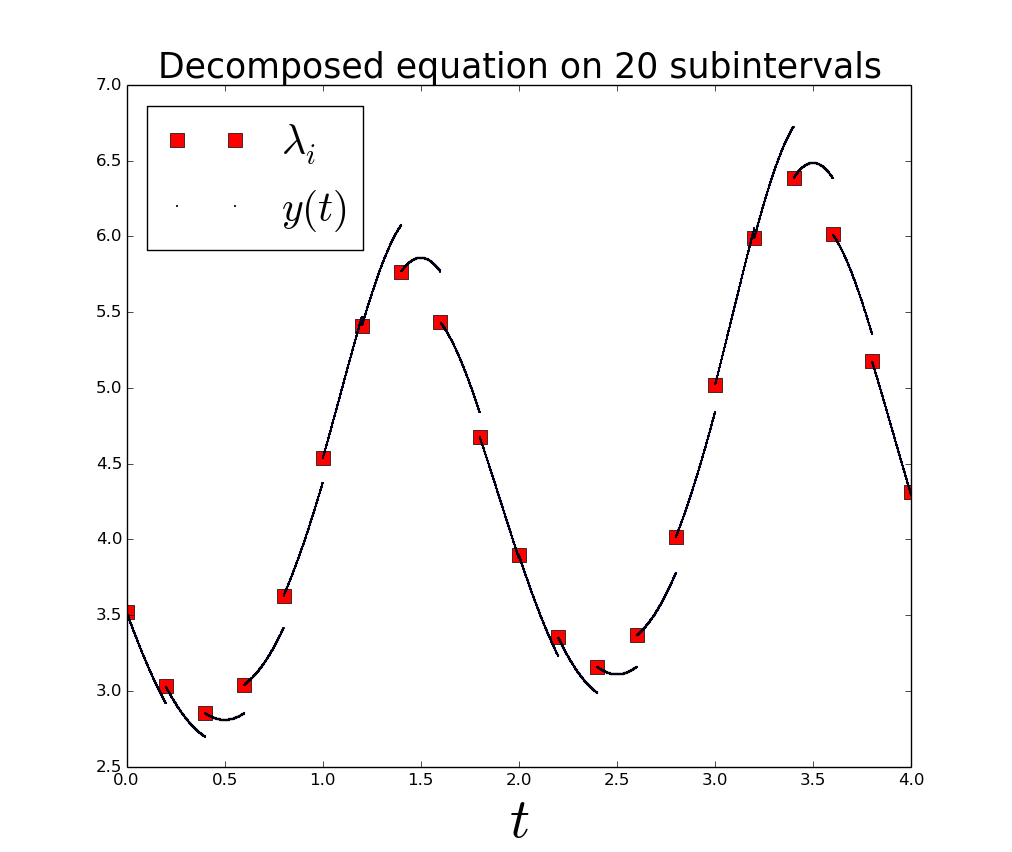
\includegraphics[scale=0.2]{parareal.png}
\caption{{\small 
The intermediate initial conditions $\{\lambda_i\}_{i=1}^{19}$ are found using a coarse solve. The fine scheme is then applied independently on each subinterval with the $\lambda_i$'s as initial conditions.
}}
\end{figure}
\end{columns}

\end{frame}

\begin{frame}
\frametitle{The reduced problem}
\begin{itemize}
\item{If the State equation is well posed for all control variables $v\in V$, we can define a reduced objective function $\hat{J}(v) = J(y(v),v)$.}
\item{Using $\hat J$, we can transform the optimal control problem into an unconstrained optimization problem.}
\end{itemize}
\begin{align*}
\min_{v\in V}\hat J (v)
\end{align*}
\begin{itemize}
\item{Evaluating $\hat J(v)$ requires us to first solve the state equation for the control $v$.}
\item{Since the reduced problem is unconstrained, we can use methods from unconstrained optimization to solve it. Such methods utilize the first order optimality condition $\hat J'(v)=0$, and we therefore need a way to evaluate the gradient of the reduced objective function.}
\end{itemize}
\end{frame}
\begin{frame}
\frametitle{Adjoint approach to gradient evaluation}
\begin{itemize}
\item{If $E$ and $J$ are sufficiently smooth, and $E_y$ is continuously invertible, the gradient of the reduced objective function $\hat J'(v)$ exists.}
\item{We can show that the gradient of the objective function is $\hat J'(v)=E_v(y(v),v)^*p +J_v(y(v),v)$. }
\item{$p$ is here the solution of the adjoint equation $E_y(y(v),v)^*p = J_y(y(v),v)$.}
\item{Evaluating $\hat J'$ for a control $v$ then comes down to the following three steps:}
\begin{align*}
1.\quad& \textrm{Solve the state equation $E(y,v)=0$ for $y$.}\\
2.\quad& \textrm{Solve the adjoint equation $E_y(y(v),v)^*p = J_y(y(v),v)$ for $p$.}\\
3.\quad& \textrm{Instert $y$ and $p$ into $J'(v)=E_v(y(v),v)^*p +J_v(y(v),v)$.}\\
\end{align*}
\end{itemize}
\end{frame}
\begin{frame}
\frametitle{Example problem}
\begin{columns}
\column{0.58\linewidth}
\begin{itemize}
\item<1->{Objective function:{\tiny\begin{align*}
J(y,v) = \frac{1}{2}\int_0^Tv(t)^2dt + \frac{\alpha}{2}(y(T)-y^T)^2 
\end{align*}
}%
}
\item<1->{State equation:{\tiny\begin{align*}
\left\{
     \begin{array}{lr}
       	y'(t)=ay(t) + v(t), \quad  t\in(0,T),\\
       	y(0)=y_0.
     \end{array}
   \right. 
\end{align*}
}%
}
\end{itemize}
\column{0.38\linewidth}
\begin{itemize}
\item<1->{Gradient:{\tiny
\begin{align*}
\hat{J}'(v) = v+p
\end{align*}
}%
}
\item<1->{Adjoint Equation:{\tiny
\begin{align*}
\left\{
     \begin{array}{lr}
       	p'(t)=-ap(t), \quad  t\in(0,T),\\
       	p(T)=\alpha(y(T)-y^T).
     \end{array}
   \right. 
\end{align*}
}%
}
\end{itemize}
\end{columns}
\end{frame}
%llllllllllllllllllllllllllllllllllllllllllllllll
\section{optimization}
\begin{frame}
\frametitle{Line search methods}
\begin{columns}
\column{0.58\linewidth}
\begin{itemize}
\item{Iterative methods for unconstrained optimization.}
\item{Produces iterates $\{x^k\}$, utilizing an initial guess $x^0$.}
\item{One iteration of a line search method:}
{\small
\begin{align*}
1.\quad& \textrm{Find descent direction $p^k$}\\
2.\quad& \textrm{Find an adequate step length $\gamma^k$}\\
3.\quad& \textrm{Update iterate $x^{k+1} = x^k -\gamma^k p^k$}
\end{align*}
}%
\end{itemize}
\column{0.38\linewidth}
\begin{figure}[!h]
\centering
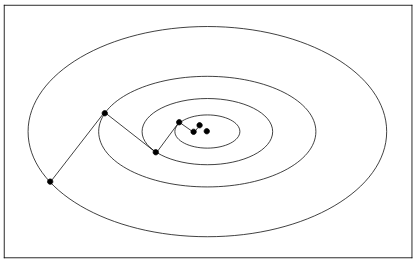
\includegraphics[scale=0.3,angle=90]{SD.png}
\end{figure}
\end{columns}
\end{frame}
\begin{frame}
\frametitle{BFGS}
\begin{itemize}
\item{Newtons method, where the descent direction is $p^k=f''(x^k)^{-1}f'(x^k)$, is a line search method that converges rapidly under strict conditions on $f''(x^k)$. }
\item{In quasi-Newton methods the search direction is instead $p^k=H^kf'(x^k)$, where $H^k\approx f''(x^k)^{-1}$. }
\item{The BFGS algorithm approximates $f''(x^k)^{-1}$ using information from previous iterates. The $H^k$'s are constructed so that it is symmetric and positive definite. To guarantee this, the initial inverted Hessian approximation $H^0$ must also possess these properties.}
\item{After each iteration $H^k$ is updated using the following formula:}
\end{itemize}
{\tiny
\begin{align*}
H^{k+1} &= (\mathbbold{1}-\rho_kS_k^T Y_k)H^k(\mathbbold{1} -\rho_kY_k^T S_k) + S_k^T S_k\\
S_k &= x^{k+1}-x^{k},
\quad Y_k = \nabla f(x^{k+1})-\nabla f(x^{k}),\\
\rho_k &= \frac{1}{Y_k^T S_k}.
\end{align*}
}%
\end{frame}
%llllllllllllllllllllllllllllllllllllllllllllllll
\section{PPC}
\begin{frame}
\frametitle{Decomposed problem}
\begin{itemize}
\item{We let $0=T_0<T_1<\cdots<T_{N-1}<T_N=T$, and decompose $[0,T]$ into $N$ subintervals $[T_{i-1},T_i]$. }
\item{We introduce intermediate initial values $\Lambda=(\lambda_1,...,\lambda_{N-1})$, and decompose the state equation into $N$ equations $E^i(y_i,v,\lambda_{i-1})=0$ defined separately on each interval $[T_{i-1},T_i]$.}
\item{To enforce continuity of the decomposed state, we introduce extra constraints $y_i(T_i)=y_{i+1}(T_i)$.}
\end{itemize}
\begin{block}{Decomposed and reduced optimal control problem}
\begin{align*}
\min_{v,\Lambda} &\hat J(v,\Lambda), \\
\textrm{subject to} \ &y_i(T_i)=\lambda_i,i=1,...,N-1. 
\end{align*}
\end{block}
\end{frame}
\begin{frame}
\frametitle{Quadratic penalty method}
\begin{columns}
\column{0.58\linewidth}
\centering
\begin{align*}
&\min_x f(x) \ \textrm{subject to} \\ &c_i(x)=0 \quad i=1,...,N
\end{align*}
Move constraints into functional:
\begin{align*}
f_{\mu}(x) = f(x) + \frac{\mu }{2}\sum_{i=1}^N c_i(x)^2 
\end{align*}
\column{0.38\linewidth}
\begin{align*}
\hat{J}_{\mu}(v,\Lambda) = \hat{J}(v) + \frac{\mu}{2}\sum_{i=1}^{N-1}(y_{i}(T_i)-\lambda_i)^2
\end{align*}
\end{columns}
\end{frame}
\begin{frame}
\frametitle{Consistency}
\begin{align*}
\lim_{\mu\rightarrow\infty} v^{\mu}=v
\end{align*}
\end{frame}
\begin{frame}
\frametitle{Parareal-based preconditioner}
\begin{align*}
(v^{k+1},\Lambda^{k+1}) = (v^k,\Lambda^k) - \rho^kH^k \hat J'(v^k,\Lambda^k)
\end{align*}
\end{frame}
\begin{frame}
\frametitle{Virtual problem}

 \begin{align}
\bold J(\Lambda) = \frac{1}{2} x(\Lambda)^Tx(\Lambda), \label{non_lin_LS}
\end{align}
\begin{align}
x(\Lambda)=\left( \begin{array}{c}  
   \lambda_1 - \bold F_{\Delta T}(\lambda_0) \\ 
   \lambda_2 - \bold F_{\Delta T}(\lambda_1) \\
   \cdots  \\
   \lambda_{N-1} -\bold F_{\Delta T}(\lambda_{N-1}) \\
   \end{array}  \right).
\end{align}

\end{frame}
%llllllllllllllllllllllllllllllllllllllllllllllllll
\section{consistency}
\begin{frame}
\frametitle{Consistency}
\begin{figure}[!h]
\centering
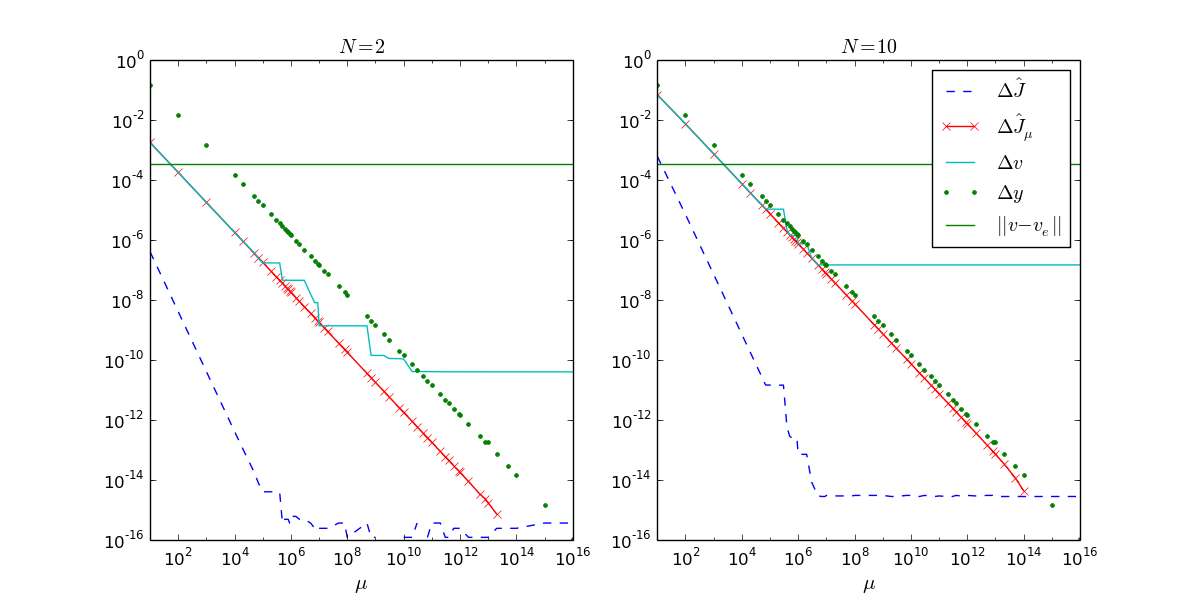
\includegraphics[scale=0.4]{consistency1.png}

\end{figure}
\end{frame}
%llllllllllllllllllllllllllllllllllllllllllllllllll
\section{Experiments}
\begin{frame}
\frametitle{Experimental setup}
\begin{itemize}
\item<1->{Total number of function and gradient evaluations for serial algorithm $L_S$ and parallel algorithm $L_{p_N}$}
\item<1->{Ideal speedup $\hat{S}=\frac{N L_S}{L_{p_N}}$}
\item<2->{$\mu$,$N$ and $n$}
\end{itemize}
\end{frame}
\end{document}

